%% This is the ctufit-thesis example file. It is used to produce theses
%% for submission to Czech Technical University, Faculty of Information Technology.
%%
%% Get the newest version from
%% https://gitlab.fit.cvut.cz/theses-templates/FITthesis-LaTeX
%%
%%
%% Copyright 2021, Eliska Sestakova and Ondrej Guth
%%
%% This work may be distributed and/or modified under the
%% conditions of the LaTeX Project Public Licenese, either version 1.3
%% of this license or (at your option) any later version.
%% The latest version of this license is in
%%  https://www.latex-project.org/lppl.txt
%% and version 1.3 or later is part of all distributions of LaTeX
%% version 2005/12/01 or later.
%%
%% This work has the LPPL maintenance status `maintained'.
%%
%% The current maintainer of this work is Ondrej Guth.
%% Contact ondrej.guth@fit.cvut.cz for bug reports.
%% Alternatively, submit bug reports into the tracker at
%% https://gitlab.fit.cvut.cz/theses-templates/FITthesis-LaTeX/issues
%%
%%

%%%%%%%%%%%%%%%%%%%%%%%%%%%%%%%%%%%%%%%%%
% CLASS OPTIONS
% language: czech/english/slovak
% thesis type: bachelor/master/dissertation
%%%%%%%%%%%%%%%%%%%%%%%%%%%%%%%%%%%%%%%%%
\documentclass[english,master,unicode]{ctufit-thesis}

%%%%%%%%%%%%%%%%%%%%%%%%%%%%%%%%%%
% FILL IN THIS INFORMATION
%%%%%%%%%%%%%%%%%%%%%%%%%%%%%%%%%%
\ctufittitle{Optimization of the painting placement problem using evolutionary techniques} % replace with the title of your thesis
\ctufitauthorfull{Bc.\,Martin Šafránek} % replace with your full name (first name(s) and then family name(s) / surname(s)) including academic degrees
\ctufitauthorsurnames{Šafránek} % replace with your surname(s) / family name(s)
\ctufitauthorgivennames{Martin} % replace with your first name(s) / given name(s)
\ctufitsupervisor{doc.\,RNDr\,Ing\,Marcel Jiřina,\,Ph.D.} % replace with name of your supervisor/advisor (include academic degrees)
\ctufitdepartment{Department of Applied Mathematics} % replace with the department of your defence
\ctufityear{2023} % replace with the year of your defence
\ctufitdeclarationplace{Prague} % replace with the place where you sign the declaration
\ctufitdeclarationdate{\today} % replace with the date of signature of the declaration
\ctufitabstractCZE{Fill in abstract of this thesis in Czech language. Class aptent taciti sociosqu ad litora torquent per conubia nostra, per inceptos hymenaeos. Cras pede libero, dapibus nec, pretium sit amet, tempor quis. Sed vel lectus. Donec odio tempus molestie, porttitor ut, iaculis quis, sem. Suspendisse sagittis ultrices augue.}
\ctufitabstractENG{Fill in abstract of this thesis in English language. Class aptent taciti sociosqu ad litora torquent per conubia nostra, per inceptos hymenaeos. Cras pede libero, dapibus nec, pretium sit amet, tempor quis. Sed vel lectus. Donec odio tempus molestie, porttitor ut, iaculis quis, sem. Suspendisse sagittis ultrices augue.}
\ctufitkeywordsCZE{enter, commma, separated, list, of, keywords, in, CZECH}
\ctufitkeywordsENG{enter, commma, separated, list, of, keywords, in, ENGLISH}
%%%%%%%%%%%%%%%%%%%%%%%%%%%%%%%%%%
% END FILL IN
%%%%%%%%%%%%%%%%%%%%%%%%%%%%%%%%%%

%%%%%%%%%%%%%%%%%%%%%%%%%%%%%%%%%%
% CUSTOMIZATION of this template
% Skip this part or alter it if you know what you are doing.
%%%%%%%%%%%%%%%%%%%%%%%%%%%%%%%%%%

\RequirePackage{iftex}[2020/03/06]
\iftutex % XeLaTeX and LuaLaTeX
\RequirePackage{ellipsis}[2020/05/22] %ellipsis workaround for XeLaTeX
\else
\RequirePackage[utf8]{inputenc}[2018/08/11] %this file encoding
\RequirePackage{lmodern}[2009/10/30] % vector flavor of Computer Modern font
\fi

% hyperlinks
\RequirePackage[pdfpagelayout=TwoPageRight,colorlinks=false,allcolors=decoration,pdfborder={0 0 0.1}]{hyperref}[2020-05-15]

% uncomment the following to hide all hyperlinks
% \RequirePackage[pdfpagelayout=TwoPageRight,hidelinks]{hyperref}[2020-05-15]

\RequirePackage{pdfpages}[2020/01/28]

\setcounter{secnumdepth}{4} % numbering sections; 4: subsubsection


%%%%%%%%%%%%%%%%%%%%%%%%%%%%%%%%%%
% CUSTOMIZATION of this template END
%%%%%%%%%%%%%%%%%%%%%%%%%%%%%%%%%%


%%%%%%%%%%%%%%%%%%%%%%
% DEMO CONTENTS SETTINGS
% You may choose to modify this part.
%%%%%%%%%%%%%%%%%%%%%%
\usepackage{dirtree}
\usepackage{lipsum,tikz}
\usepackage{csquotes}
\usepackage[style=iso-numeric]{biblatex}
\addbibresource{text/bib-database.bib}
\usepackage{listings} % typesetting of sources
% \usepackage{minted} % typesetting of sources

%theorems, definitions, etc.
\theoremstyle{plain}
\newtheorem{theorem}{Věta}
\newtheorem{lemma}[theorem]{Tvrzení}
\newtheorem{corollary}[theorem]{Důsledek}
\newtheorem{proposition}[theorem]{Návrh}
\newtheorem{definition}[theorem]{Definice}
\theoremstyle{definition}
\newtheorem{example}[theorem]{Příklad}
\theoremstyle{remark}
\newtheorem{note}[theorem]{Poznámka}
\newtheorem*{note*}{Poznámka}
\newtheorem{remark}[theorem]{Pozorování}
\newtheorem*{remark*}{Pozorování}
\numberwithin{theorem}{chapter}
%theorems, definitions, etc. END
%%%%%%%%%%%%%%%%%%%%%%
% DEMO CONTENTS SETTINGS END
%%%%%%%%%%%%%%%%%%%%%%

\usepackage{graphicx}
\graphicspath{{figures/}}

% big tables & rotating page
\usepackage{pdflscape}
\usepackage{afterpage}

\usepackage[export]{adjustbox}
%% for aligning: \includegraphics[width=.6\textwidth,left]{example-image}

\usepackage{todonotes}
\usepackage{amsmath}
\usepackage{amsfonts}

% Enable subfloats within figures
\usepackage{subfig}

%%%%%%%%%%%%%%%%%%%%%%%%%%%%%%%%%%%%%%
% VLASTNI MAKRA
%%%%%%%%%%%%%%%%%%%%%%%%%%%%%%%%%%%%%%

\def\todoc{\todo[color=yellow]{cite}}
\def\todoi#1{\todo[inline, color=green]{#1}}
\newcommand{\navesti}[1]{\noindent\textbf{\textit{{#1}}}}
\DeclareMathOperator*{\argmax}{arg\,max}
\DeclareMathOperator*{\argmin}{arg\,min}
\DeclareMathOperator*{\real}{\mathbb{R}}
\DeclareMathOperator*{\realpos}{\mathbb{R}^+}
\DeclareMathOperator*{\nat}{\mathbb{N}}
\DeclareMathOperator*{\natpos}{\mathbb{N}^+}

\begin{document}
    \frontmatter\frontmatterinit % do not remove these two commands

    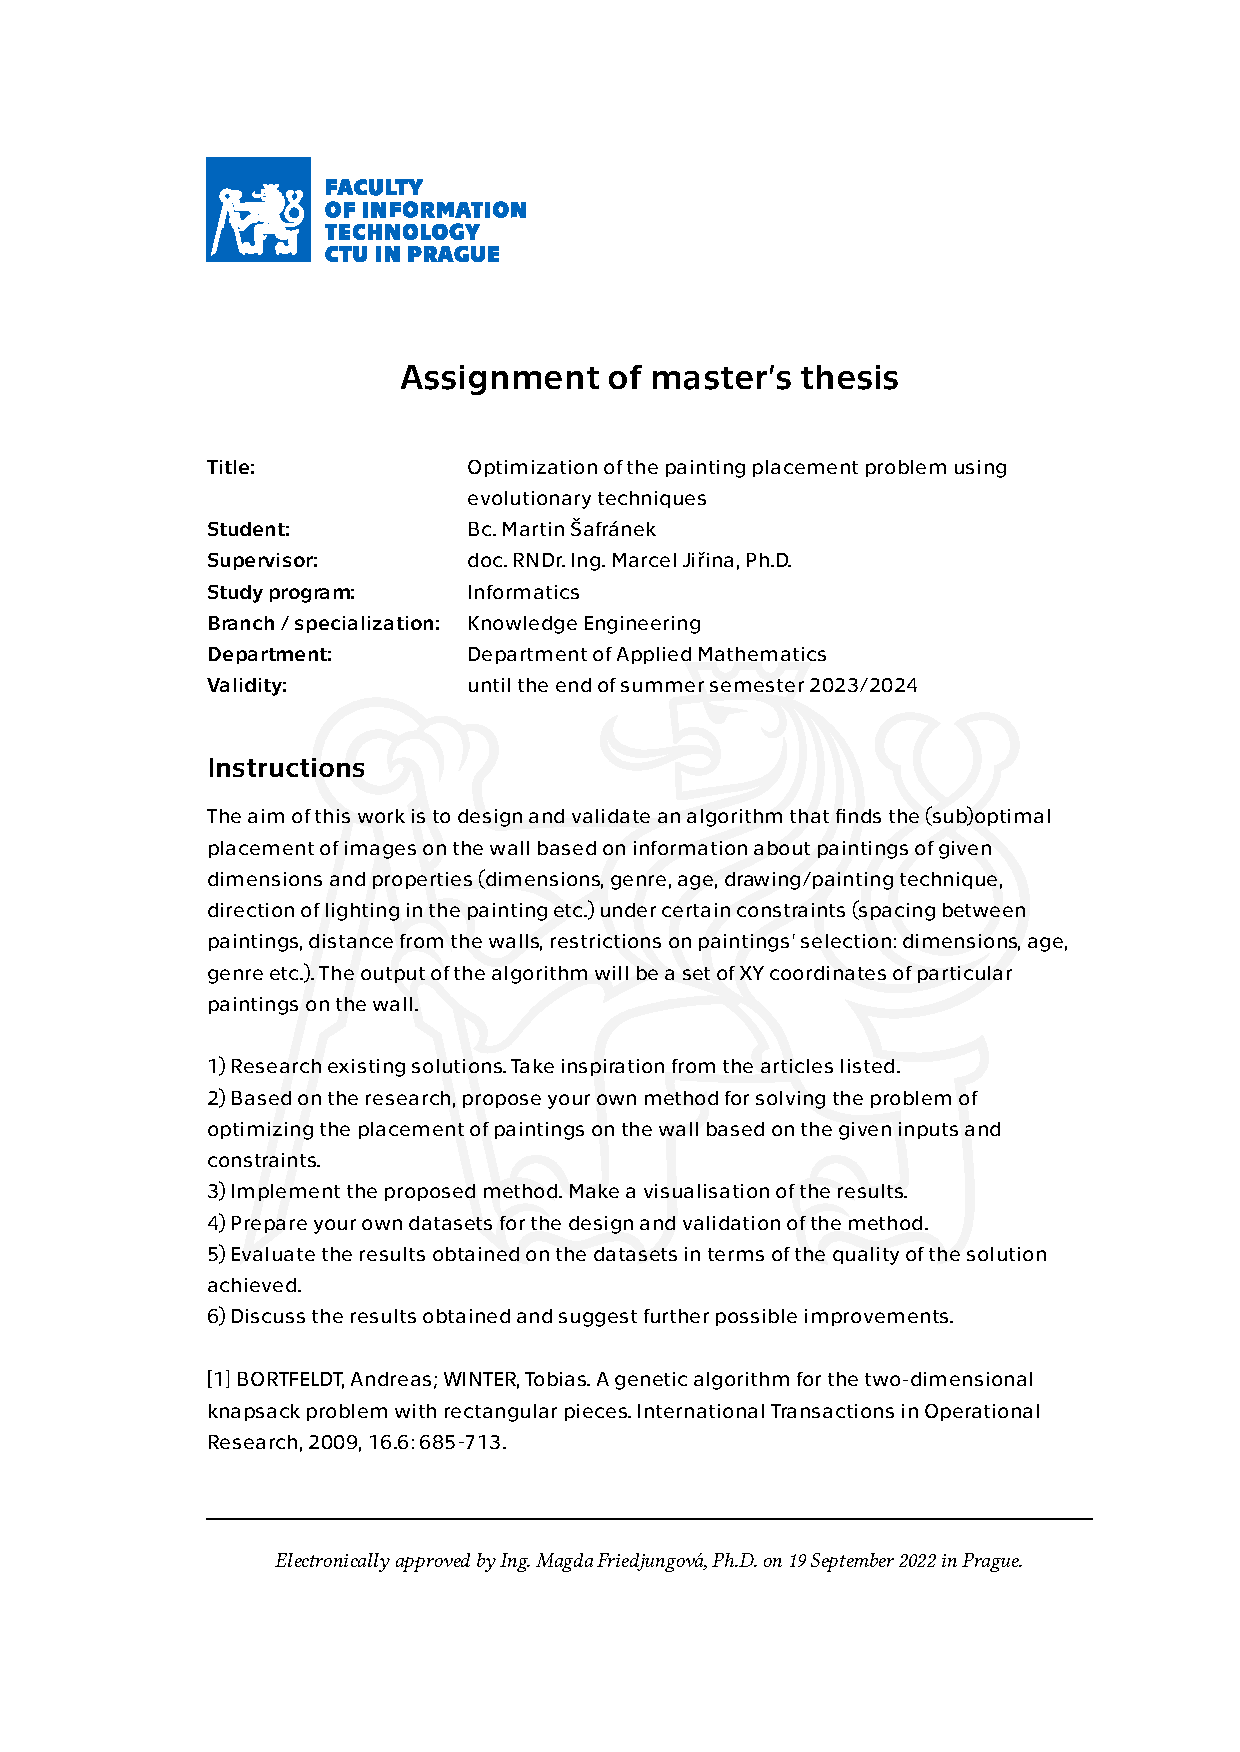
\includepdf[pages={1-}]{assignment-include.pdf} % replace that file with your thesis assignment provided by study office

    \thispagestyle{empty}\cleardoublepage\maketitle % do not remove these three commands

    \imprintpage % do not remove this command

    \tableofcontents % do not remove this command
%%%%%%%%%%%%%%%%%%%%%%
% list of other contents: figures, tables, code listings, algorithms, etc.
% add/remove commands accordingly
%%%%%%%%%%%%%%%%%%%%%%
    \listoffigures % list of figures
    \begingroup
    \let\clearpage\relax
    \listoftables % list of tables
    \lstlistoflistings % list of source code listings generated by the listings package
% \listoflistings % list of source code listings generated by the minted package
    \endgroup
%%%%%%%%%%%%%%%%%%%%%%
% list of other contents END
%%%%%%%%%%%%%%%%%%%%%%

%%%%%%%%%%%%%%%%%%%
% ACKNOWLEDGMENT
% FILL IN / MODIFY
% This is a place to thank people for helping you. It is common to thank your supervisor.
%%%%%%%%%%%%%%%%%%%
    \begin{acknowledgmentpage}
        Chtěl bych poděkovat především sit amet, consectetuer adipiscing elit. Curabitur sagittis hendrerit ante. Class aptent taciti sociosqu ad litora torquent per conubia nostra, per inceptos hymenaeos. Cras pede libero, dapibus nec, pretium sit amet, tempor quis. Sed vel lectus. Donec odio tempus molestie, porttitor ut, iaculis quis, sem. Suspendisse sagittis ultrices augue.
    \end{acknowledgmentpage}
%%%%%%%%%%%%%%%%%%%
% ACKNOWLEDGMENT END
%%%%%%%%%%%%%%%%%%%


%%%%%%%%%%%%%%%%%%%
% DECLARATION
% FILL IN / MODIFY
%%%%%%%%%%%%%%%%%%%
% INSTRUCTIONS
% ENG: choose one of approved texts of the declaration. DO NOT CREATE YOUR OWN. Find the approved texts at https://courses.fit.cvut.cz/SFE/download/index.html#_documents (document Declaration for FT in English)
% CZE/SLO: Vyberte jedno z fakultou schvalenych prohlaseni. NEVKLADEJTE VLASTNI TEXT. Schvalena prohlaseni najdete zde: https://courses.fit.cvut.cz/SZZ/dokumenty/index.html#_dokumenty (prohlášení do ZP)
    \begin{declarationpage}
        I hereby declare that the presented thesis is my own work and that I have cited all
        sources of information in accordance with the Guideline for adhering to ethical
        principles when elaborating an academic final thesis.
        I have used Grammarly to correct minor spelling issues and ChatGPT to assist me with writing Python code that generates graphs. \todo{nechat tuhle jednu vetu zde nebo dat do podekovani?}

        I acknowledge that my thesis is subject to the rights and obligations stipulated by the
        Act No. 121/2000 Coll., the Copyright Act, as amended, in particular that the Czech
        Technical University in Prague has the right to conclude a license agreement on the
        utilization of this thesis as a school work under the provisions of Article 60 (1) of the
        Act.
    \end{declarationpage}
%%%%%%%%%%%%%%%%%%%
% DECLARATION END
%%%%%%%%%%%%%%%%%%%

    \printabstractpage % do not remove this command

%%%%%%%%%%%%%%%%%%%
% SUMMARY
% FILL IN / MODIFY
% OR REMOVE ENTIRELY (upon agreement with your supervisor)
% (appropriate to remove in most theses)
%%%%%%%%%%%%%%%%%%%
%    \begin{summarypage}
%        \section*{Summary section}
%
%        \lipsum[1][1-8]
%
%        \section*{Summary section}
%
%        \lipsum[2][1-6]
%
%        \section*{Summary section}
%
%        \lipsum[3]
%
%        \section*{Summary section}
%
%        \lipsum[2]
%
%        \section*{Summary section}
%
%        \lipsum[1][1-8] Lorem lorem lorem.
%    \end{summarypage}
%%%%%%%%%%%%%%%%%%%
% SUMMARY END
%%%%%%%%%%%%%%%%%%%

%%%%%%%%%%%%%%%%%%%
% ABBREVIATIONS
% FILL IN / MODIFY
% OR REMOVE ENTIRELY
% List the abbreviations in lexicography order.
%%%%%%%%%%%%%%%%%%%


    \chapter{Acronyms}

    \todo{sort alphabetically}
    \begin{tabular}{rl}
        2D-KP   & Two-Dimensional Knapsack             \\
        BL      & Bottom Left                          \\
        BL-F    & TODO                                 \\
        BRKGA   & Biased Random Key Genetic Algorithm  \\
        FLP     & Facility Layout Problem              \\
        GA      & Genetic Algorithm                    \\
        QAP     & Quadratic Assignment Problem         \\
        RKGA    & Random Key Genetic Algorithm         \\
        UA-FLP  & Unequal Area Facility Layout Problem \\
        NP-hard & TODO                                 \\
        I/O     & TODO                                 \\
    \end{tabular}
%%%%%%%%%%%%%%%%%%%
% ABBREVIATIONS END
%%%%%%%%%%%%%%%%%%%

    \mainmatter\mainmatterinit % do not remove these two commands

%%%%%%%%%%%%%%%%%%%
% THE THESIS
% MODIFY ANYTHING BELOW THIS LINE
%%%%%%%%%%%%%%%%%%%

    \chapter{Literature overview}\label{ch:literature-overview}

In \cite{kandasamyEffectiveLocationMicro2020} authors proposed solution to cutting problem.
They describe it as cutting multiple parts from metal sheet using cutting tool.
The main focus is on preventing cutted parts from falling out of the metal sheet.
They use micro-joints to solve this problem. Micro-joint is part of the cutting tool
path that is not cutted – holding part and preventing it from falling.

This presents multitude of problems that they address by using genetic algorithm
and heuristic. Chromosome is genetic string with two parts – first holds
angle values and second holds segment numbers. Using this representation they are able
to map (using simple heuristic) each individual to one cutting tool path and micro-joint positions.
Fitness and objective are minimize air travel distance for the cutting tool needed to cut the
path. They used standard operators – two point partial matching crossover and mutation
as swapping chromosome genes.

According to the authors they achieved "near optimal" results in comparison with randomly
generated solutions and industry standards for cutting sheet metal parts.

In \cite{vijayanandHeuristicGeneticApproach2015} authors solved similar problem. They it
as placing squares to the grid with two optimization criterions – minimize air travel distance
for the cutting tool needed to cut the path (same as above), minimize unused are of the grid (different from above).
Formulation of this problem is closely related to 2SLOPP\footnotemark

WIP: Summary of "Review of the cutting path algorithms" \cite{dewilReviewCuttingPath2016}.


\begin{figure}[htp]
    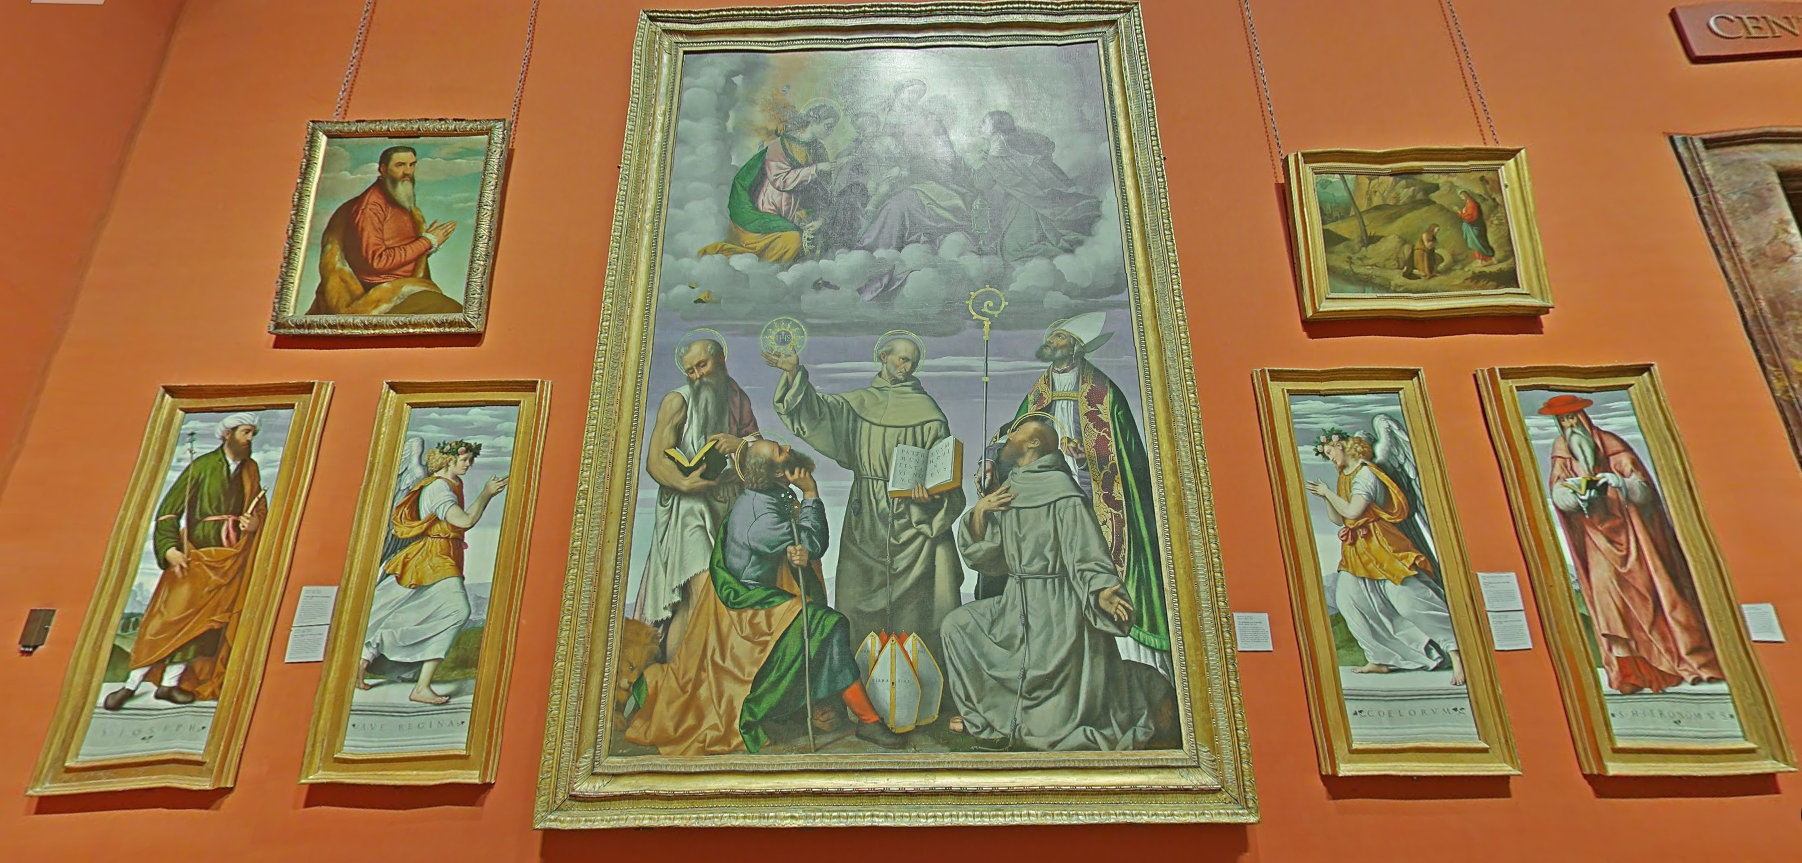
\includegraphics[width=1\textwidth, left]{london_gallery_wall}
    \caption{Painting placement at the The National Gallery, London. Source:~\cite{ScreenshotWallGoogle}}
    \label{fig:london-wall}
\end{figure}

\footnotetext{Two dimensional single large object placement problem}


\chapter{Coding}\label{ch:coding}


\begin{figure}[htp]
    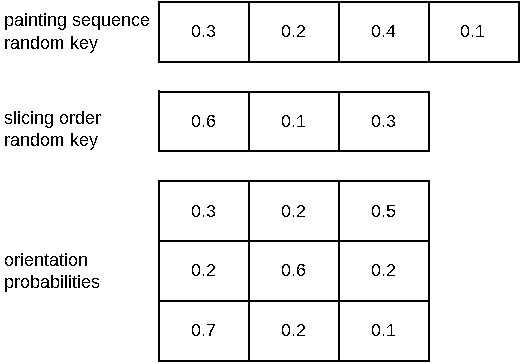
\includegraphics[width=1.0\textwidth, center]{chromosome}\label{fig:chromosome}
    \caption{
        Example of an individual representation – 3D chromosome composed of two random key vectors
        and one matrix, whose rows are also random keys.
        Each vector and matrix row form a probability distribution, i.e., they sum up to 1.
    }
\end{figure}

\begin{figure}[htp]
    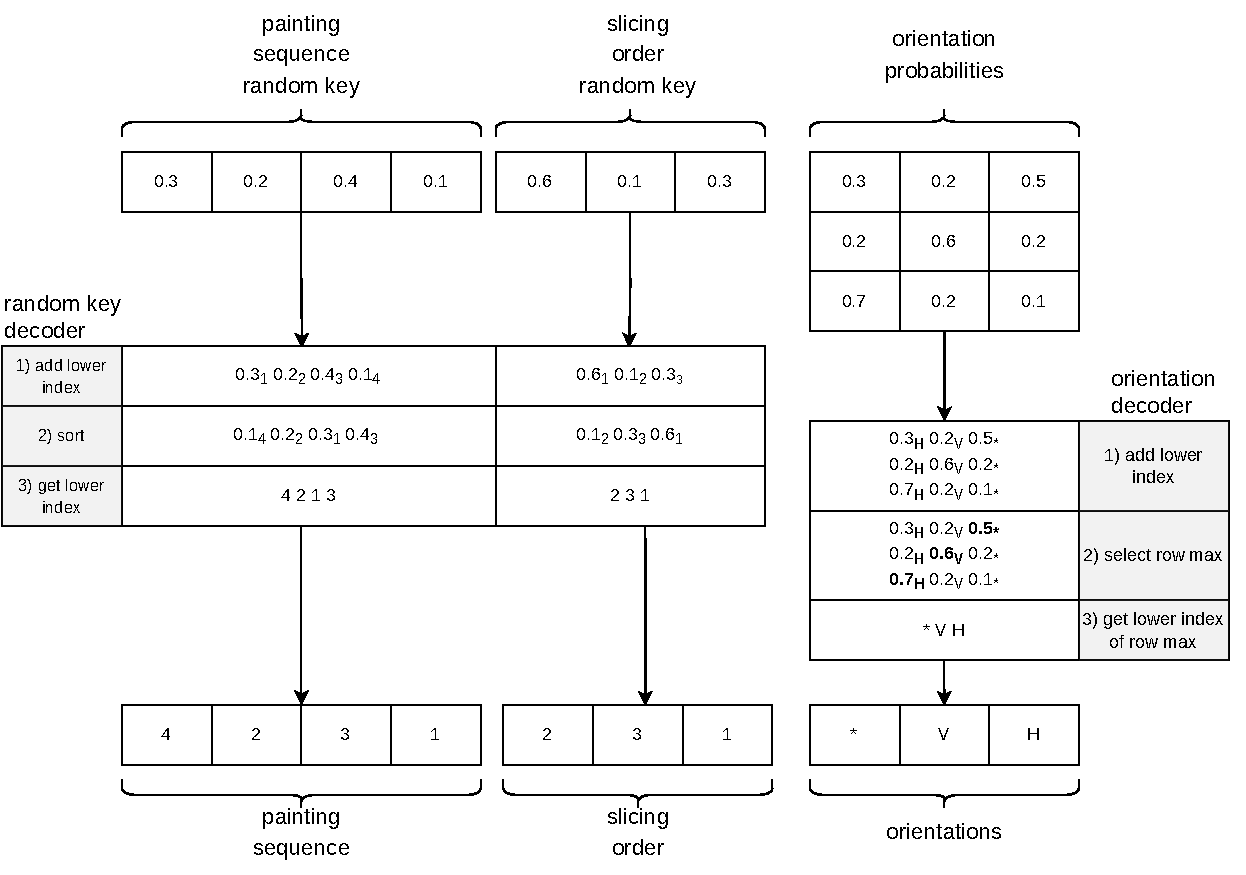
\includegraphics[width=1.1\textwidth, left]{individual_decoding}
    \caption{
        Individual decoding example. Both the painting sequence random key and slicing order random key
        are decoded using the same procedure. The decoded individual can be used to construct a slicing layout.
    }
    \label{fig:individual-decoding}
\end{figure}

\begin{figure}[htp]
    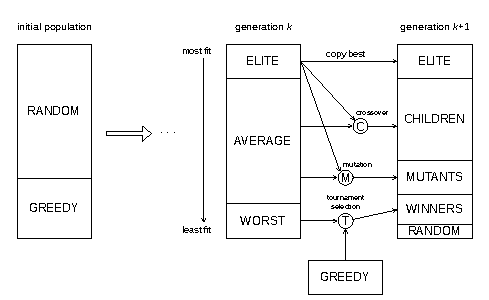
\includegraphics[width=1.1\textwidth, left]{pupulation_schema}\label{fig:population-schema}
    \caption{Initial population generation strategy and transition from generation $k$ to $k+1$.}
\end{figure}


\section{Operators}\label{sec:operators}
This sections describes operators – actions on the individual representation
seen in section~\ref{subsec:individual-representation}.

We can guide the genetic search in two basic ways – diversification and intensification.
If the diversification is high, the search process is biased towards exploring genomes
that may be vastly different from the one already present in the population.
This tries to prevent the genetic search from getting stuck in a local optimum.
Diversification that is too high would reassemble a random walk, ultimately randomly sampling
from the space of all possible genomes. On the other hand, if the intensification is high,
biased towards exploiting similar genemos takes precedence.

It is crucial to find the correct balance between diversification and intensification.
One way to control the diversification in genetic algorithm is setting
mutation probability – high chance of mutation means higher diversification, low change is the opposite.
Intensification can be similarly controller by the crossover probability.
\ref{TODO}

\subsection{Mutation}\label{subsec:mutation}
Mutation takes place on all 3 parts of a chromosome, as seen in example in table \ref{tab:ind-rep-example}.
Since both random keys vectors and orientation probabilities form a probability distribution vector,
it is easy to perform mutation by replacing a value with a randomly generated one from interval $[0,1]$
and then normalize back to the probability distribution.

For example, consider $$[0.6, 0.1, 0.3]$$ be a painting sequence random key or slicing order random key.
Mutation operator would randomly choose one position in the vector, say the first one, and replace it
with a randomly generated one from interval $[0,1]$. The result may be $$[0.9, 0.1, 0.3]$$.
The mutated vector forms no longer a probability distribution and to obtain the mutated value
it needs to be normalized – finally ending up with $[0.7, 0.07, 0.23]$.

Mutation for the orientation probabilities is the same but with the first additional
step of randomly choosing which of the probability vectors will undergo the aforementioned process.

\begin{figure}[htp]
    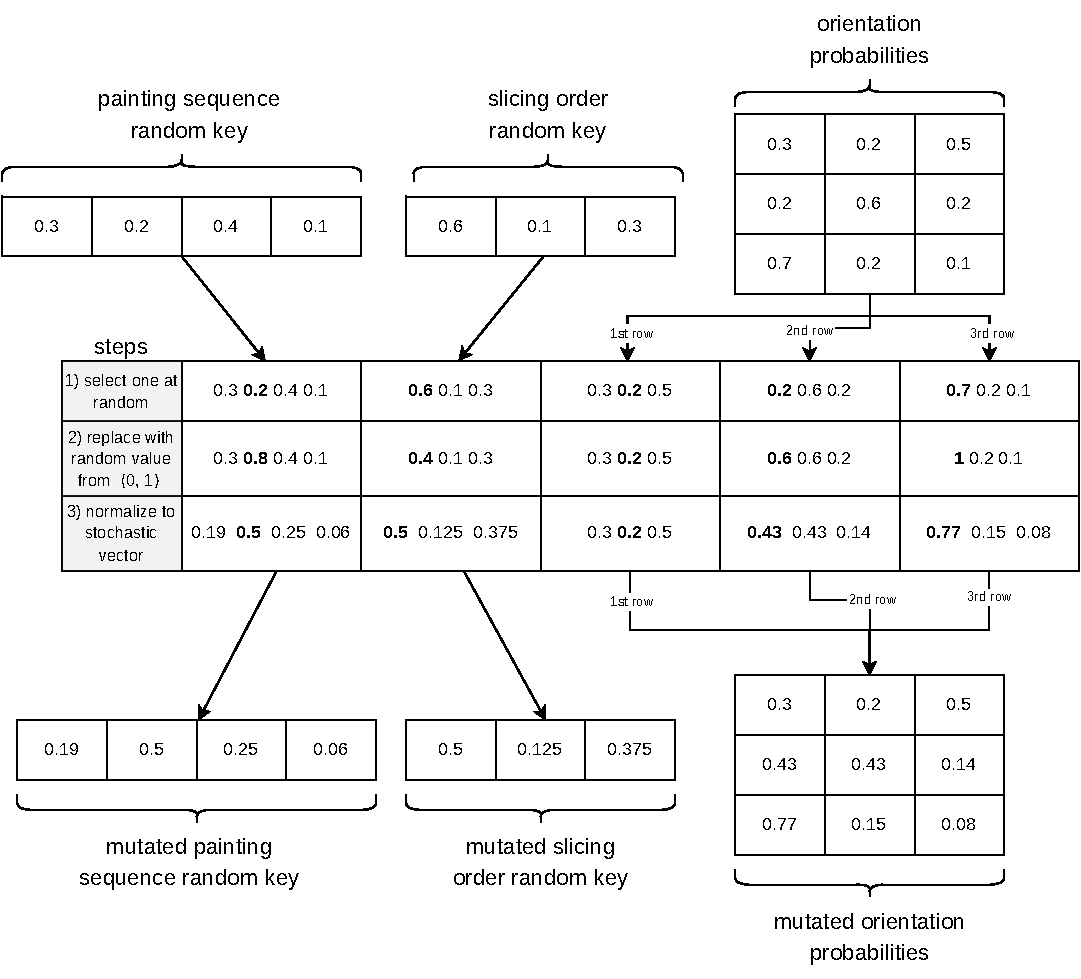
\includegraphics[width=1.0\textwidth, left]{muation}\caption{
        Example of a mutation on all three parts of a chromosome.
        Since all parts can be treated as a random key, only one procedure
        is used – replace one value at random and then normalize to a stochastic vector.
    }
    \label{fig:mutation}
\end{figure}

\subsection{Crossover}\label{subsec:crossover}

\begin{figure}[htp]
    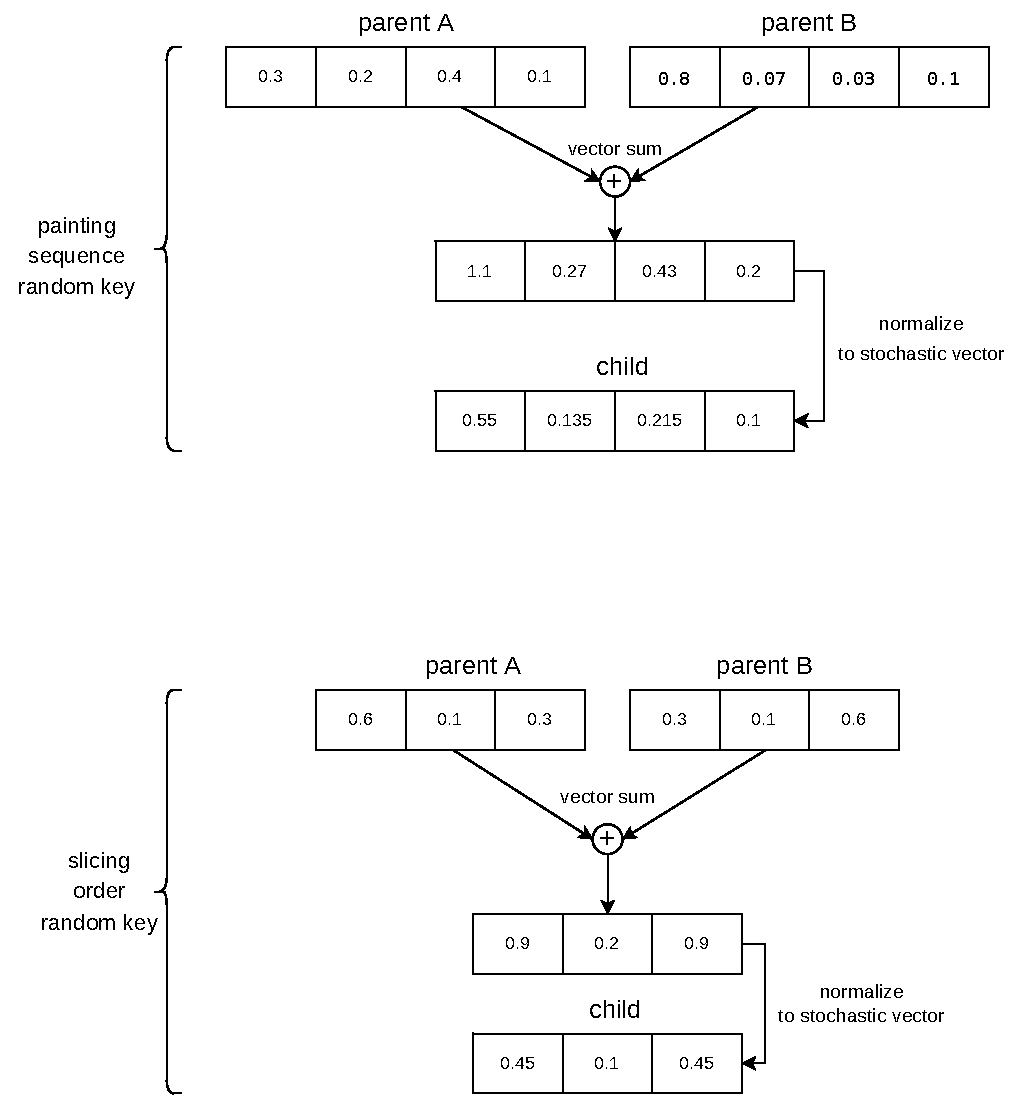
\includegraphics[width=1.1\textwidth, left]{crossover_random_keys}\caption{
        Crossover example for painting sequence and slicing order random keys.
        The procedure is the same for both – sum parent vectors and then normalize to stochastic vector.
    }
    \label{fig:crossover-random-keys}
\end{figure}

\begin{figure}[htp]
    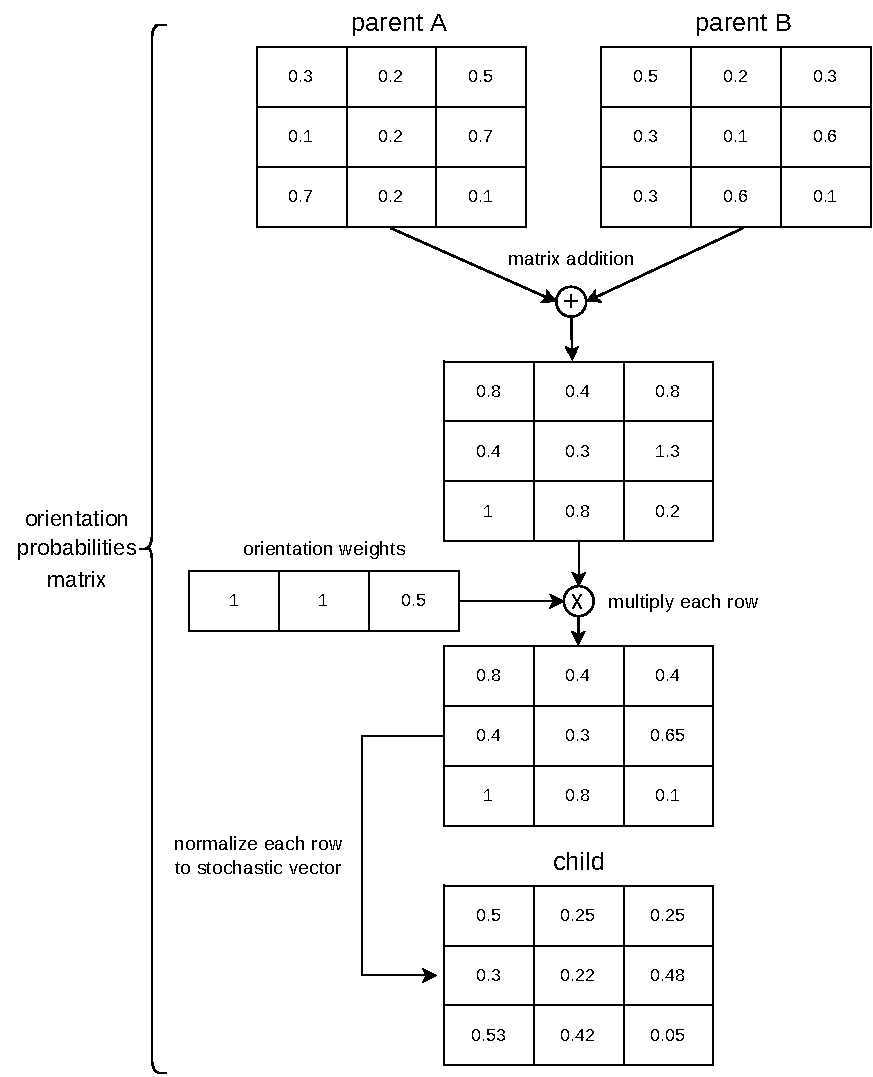
\includegraphics[width=0.85\textwidth, left]{crossover_orientation_probabilities}\caption{
        Crossover example for orientation probabilities. The procedure is first to sum parent matrices,
        then weight each row with orientation weights and normalize each row to a stochastic vector.}
    \label{fig:crossover-orientation-probabilities}
\end{figure}



 % include `text.tex' from `text/' subdirectory

    \printbibliography % print out the BibLaTeX-generated bibliography list

    \appendix\appendixinit % do not remove these two commands

    \chapter{Appendix}\label{ch:appendix}


\begin{listing}[h!]
    \centering
    \begin{cminted}[autogobble,breaklines=true]{shell}
        $ curl --location 'localhost:9000/compute' \
        --header 'Content-Type: application/json' \
        --data '{
            "instanceParameters": {
                "layout": {
                    "width": 30,
                    "height": 20,
                    "evalFunc": "f(x,y) = x+y"
                },
                "paintings": [
                    { "ident": "1", "width": 5, "height": 7 },
                    { "ident": "2", "width": 5, "height": 7 },
                    { "ident": "3", "width": 5, "height": 7 },
                    { "ident": "4", "width": 5, "height": 7 },
                    { "ident": "5", "width": 5, "height": 7 },
                    { "ident": "6", "width": 5, "height": 7 }
                ],
                "paintingsFlow": [
                    { "from": 1, "to": 2, "flow": 3.3 },
                    { "from": 1, "to": 3, "flow": 4.4 },
                    { "from": 1, "to": 5, "flow": 0 }
                ]
            },
            "gaParameters": {
                "maxNumberOfIter": 2,
                "populationSize": 100,
                "maximumWildCardCount": 1,
                "orientationWeights": [ 1, 1, 0.5 ],
                "geneticAlgorithm": "simpleGa",
                "mate": "normalizedProbabilityVectorSum",
                "mutate": "flipOnePartAtRandom",
                "select": "tournament",
                "objective": "simple",
                "evaluator": "ga",
                "placingHeuristics": "corner",
                "populationDivisionCounts": {
                    "elite": 0.2, "average": 0.6, "worst": 0.2,
                    "children": 0.3, "mutant": 0.2, "winner": 0.2,
                    "random": 0.1
                },
                "initialPopulationDivisionCounts": {
                    "random": 0.7, "greedy": 0.3
                }
            },
            "objectiveParameters": {
                "name": "simple",
                "params": {
                    "overlappingPenalizationConstant": 1000,
                    "outsideOfAllocatedAreaPenalizationConstant": 0
                }
            }
        }'
    \end{cminted}
    \cprotect\caption[Example of computation submission without instance.]{Example of computation submission using \verb|curl|\footnotemark[1] without specyfing the instance name.
    Without it, everything has to be entered manually into the request – layout width and height, paintings together with their flow and evaluation function.}

    \label{lst:computation-submission-manual}
\end{listing}

\footnotetext[1]{\url{https://curl.se/}}
 % include `appendix.tex' from `text/' subdirectory

    \backmatter % do not remove this command

    \chapter{Contents of the attached medium}


	\dirtree{%
		.1 README.md\DTcomment{the file with attached medium contents description}.
		.1 impl\DTcomment{the directory with implementation source code}.
		.2 public/datasets\DTcomment{the directory of datasets}.
		.1 notebooks\DTcomment{the directory of Jupyter notebooks for visualization and dataset generation}.
		.1 thesis\DTcomment{the directory with thesis}.
		.2 ctufit-thesis-en.tex\DTcomment{the thesis source in TEX format}.
		.2 ctufit-thesis-en.pdf\DTcomment{the thesis text in PDF format}.
	}
 % include `medium.tex' from `text/' subdirectory

\end{document}
